\section{\Sys Design}
\label{sec:methodology}

% \begin{algorithm}[h]
%   \scriptsize
%   \DontPrintSemicolon
%   \SetKwInOut{Input}{Inputs}
%   \SetKwInOut{Output}{Output}
%   \Input{Set of client models $\{M_1, M_2, \ldots, M_N\}$;\\}
%   \Output{Global GNN model $G$.}
%   \BlankLine
%   \tcc{Initialize global GNN model with random weights.}
%   $G \leftarrow \text{InitializeRandomWeights}()$\\
%   \tcc{Distribute $G$ to all clients.}
%   \ForEach{client model $M_i$}{
%     Send $G$ to $M_i$\\
%     $G_i \leftarrow \text{TrainOnLocalData}(M_i)$
%   }
%   \BlankLine
%   \tcc{Aggregate trained models from clients.}
%   $AggregatedWeights \leftarrow list([])$\\
%   \ForEach{client model $G_i$}{
%     $AggregatedWeights.append(\text{ExtractWeights}(G_i))$\\
%   }
%   \tcc{Apply federated averaging.}
%   $G \leftarrow \text{FederatedAveraging}(AggregatedWeights)$\\
%   \BlankLine
%   \Return $G$\\
%   \BlankLine
%   \caption{Federated Graph Representation Learning}
%   \label{alg:federated_learning}
% \end{algorithm}

\begin{algorithm}[!t]
  \scriptsize
  \DontPrintSemicolon
  \SetKwInOut{Input}{Inputs}
  \SetKwInOut{Output}{Output}
  \Input{Set of client models $\{\{M_{1,1}, M_{1,2}, \ldots, M_{1,n}\},$\\ 
  $\{M_{2,1}, M_{2,2}, \ldots, M_{2,n}\}, \ldots,$\\
  $\{M_{N,1}, M_{N,2}, \ldots, M_{N,n}\}\}$;}
  \Output{Set of global GNN models $\{G_1, G_2, \ldots, G_n\}$.}
  \BlankLine
  \tcc{Initialize global GNN models with random weights.}
  $\{G_1, G_2, \ldots, G_n\} \leftarrow \text{InitializeRandomWeightsForEachModel}(n)$\\
  \BlankLine
  \tcc{Distribute each $G_k$ to corresponding models of all clients.}
  \For{$k \leftarrow 1$ \KwTo $n$}{
    \ForEach{client model set $\{M_{i,1}, M_{i,2}, \ldots, M_{i,n}\}$}{
      Send $G_k$ to $M_{i,k}$\\
      $G_{i,k} \leftarrow \text{TrainOnLocalData}(M_{i,k})$\\
    }
  }
  \BlankLine
  \For{$k \leftarrow 1$ \KwTo $n$}{
    $AggregatedWeights_k \leftarrow list([])$\\
    \ForEach{client model $G_{i,k}$}{
      $AggregatedWeights_k.append(\text{ExtractWeights}(G_{i,k}))$\\
    }
    $G_k \leftarrow \text{FederatedAveraging}(AggregatedWeights_k)$\\
  }
  \BlankLine
  \Return $\{G_1, G_2, \ldots, G_n\}$\\
  \BlankLine
  \caption{Federated Graph Representation Learning.}
  \label{alg:federated_learning}
\end{algorithm}

In this section, we detail the architecture of \Sys, which is composed of six key modules. The architecture begins with the \textit{Provenance Graph Constructor} module on each client machine, transforming audit logs into a provenance graph. Following this, the \textit{Semantic Featurization} module encodes semantic attributes from the audit logs into feature vectors, facilitating the training of client-specific \gnnshort models.

The \textit{Semantic Vectors Harmonization} module aims to privately consolidate individual client word2vec models into a cohesive global model, employing a trusted utility server and encryption techniques to ensure the privacy of model data.

Next, the \textit{System Entity Categorization} module categorizes all system entities across clients into standardized categories, promoting uniformity in the training of \gnnshort models.

The \textit{Federated Graph Learning Module} proceeds to train \gnnshort models by these categories on each client machine, using the harmonized semantic features. After training, the models are sent to a central server for federated learning, where the federated averaging algorithm integrates the models based on the system entity categories they were trained on.

Lastly, the \textit{Anomaly Detection Module} employs the unified global models for anomaly detection on each client machine. Figure \ref{fig:arch} presents the comprehensive architecture of \Sys, with further details in the subsequent subsections:

\begin{figure*}[t!]
  \centering
  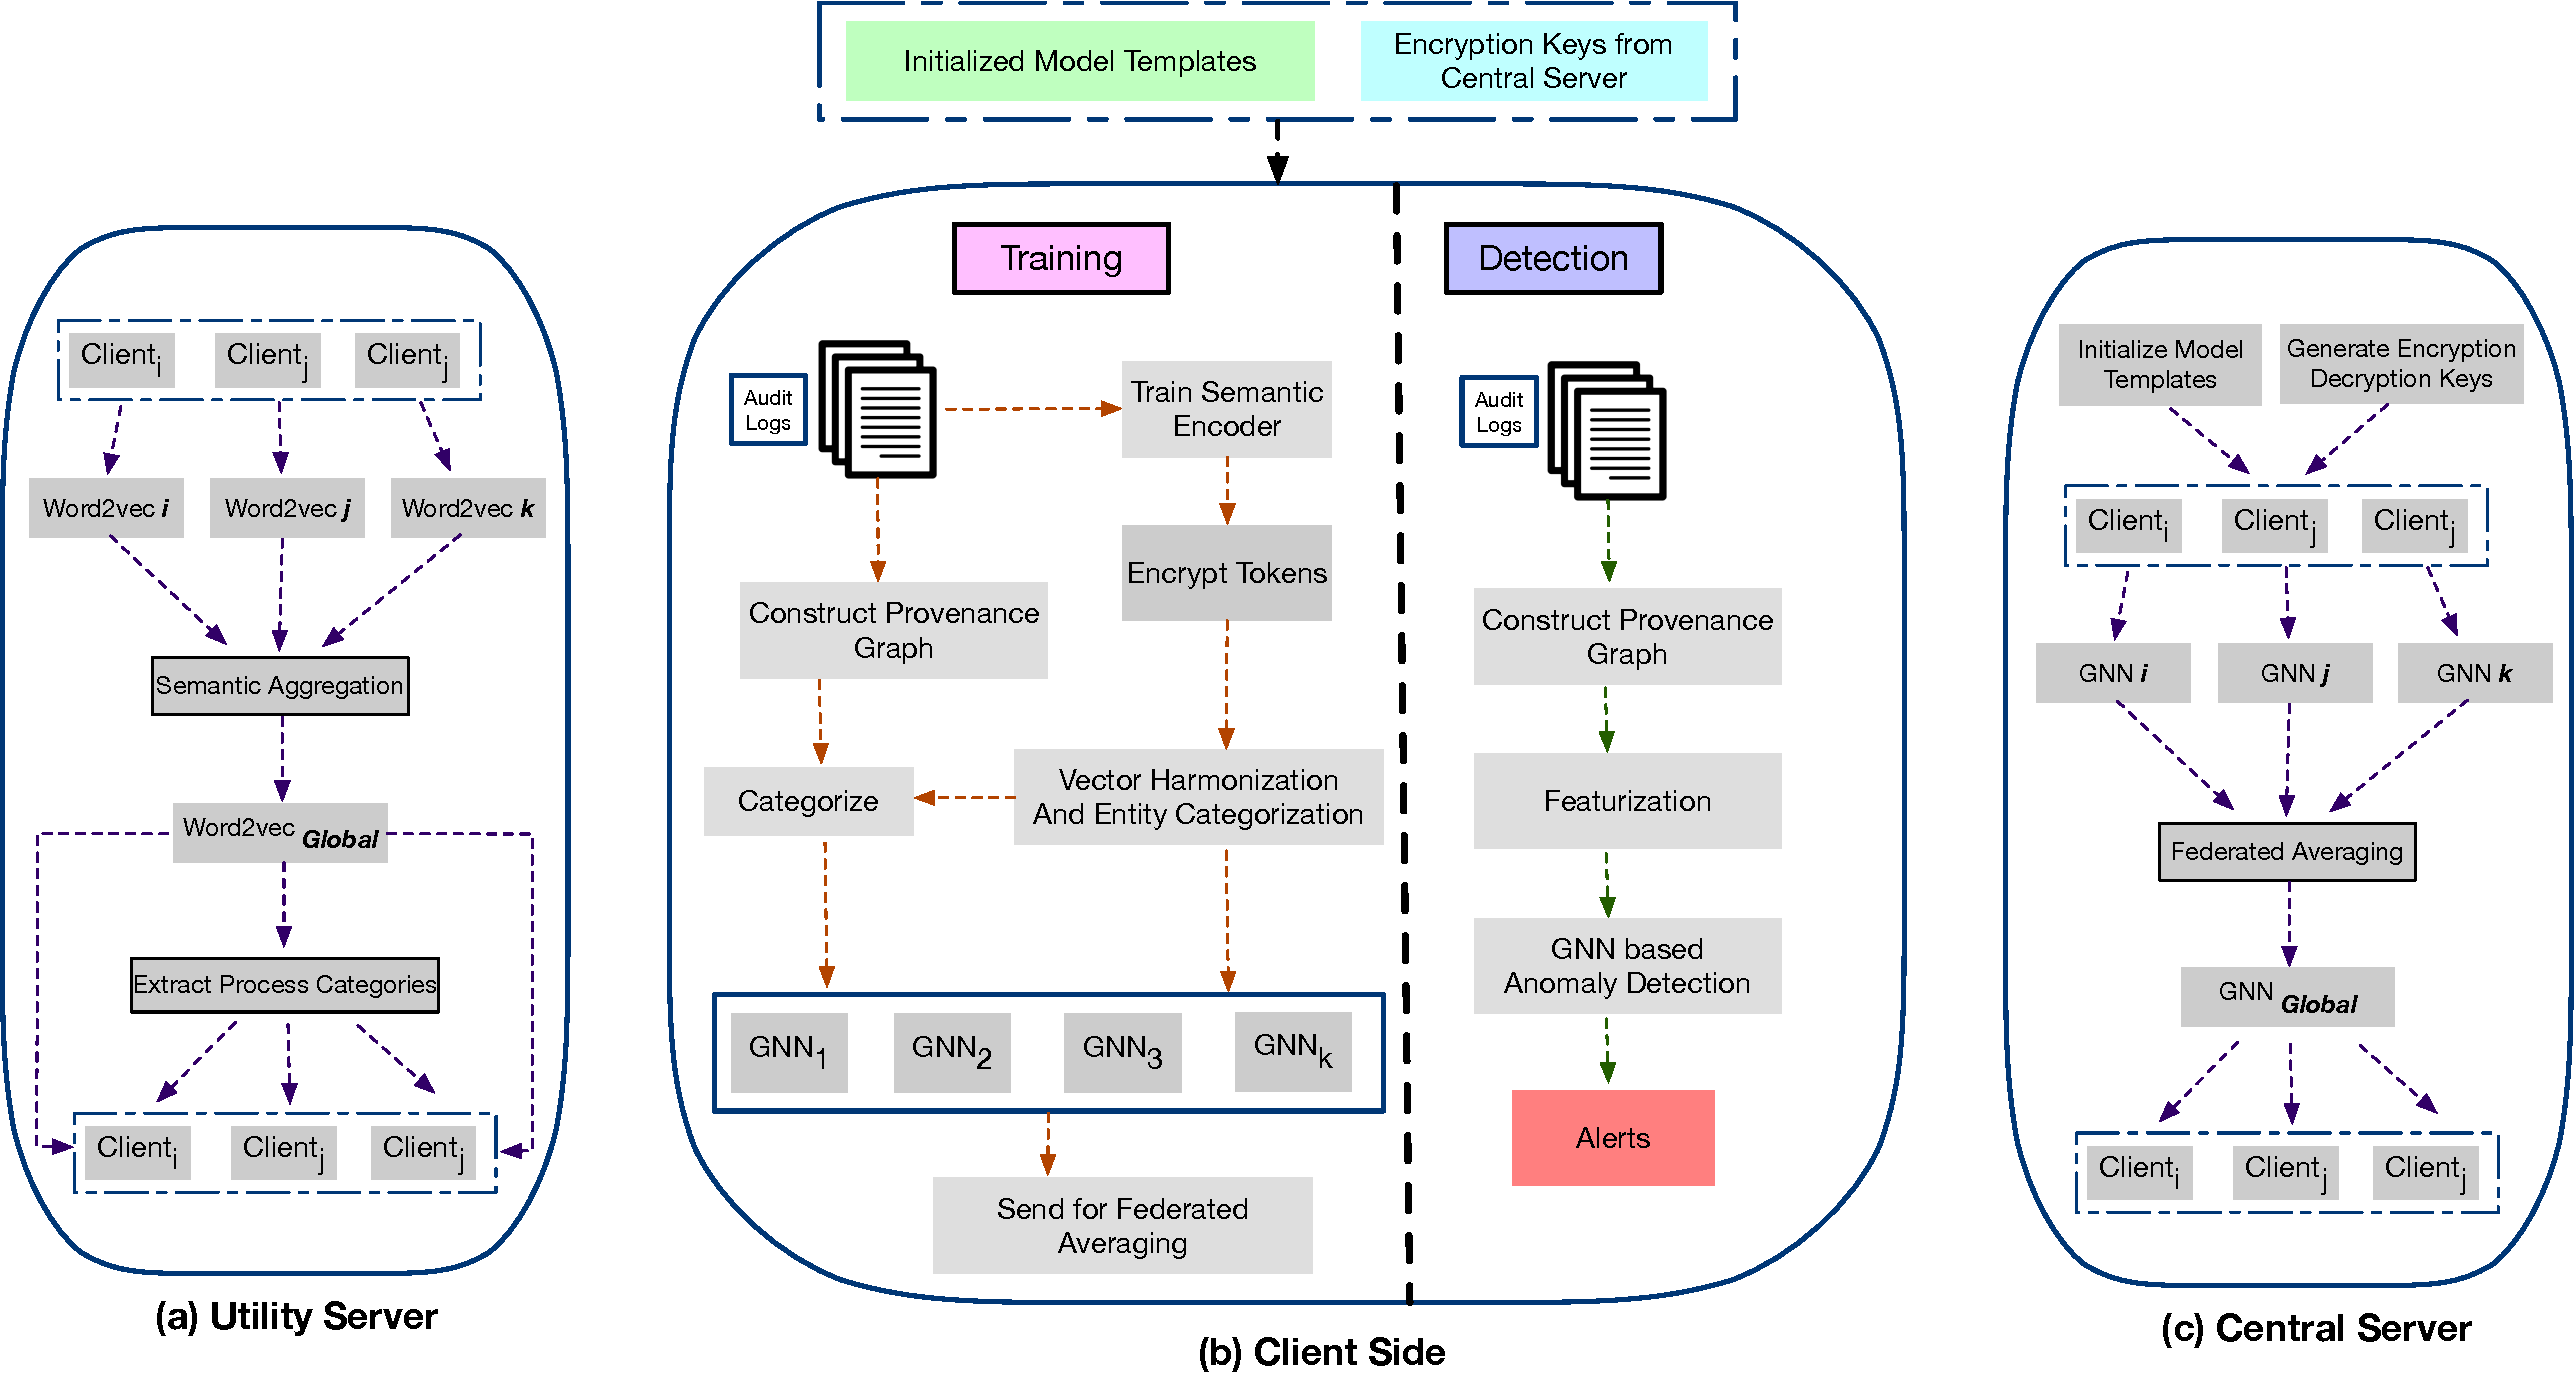
\includegraphics[width=\textwidth]{fig/archv2.pdf}
  \caption{High Level Architecture of \Sys.}
  \vspace{-3ex}
  \label{fig:arch}
\end{figure*}

\subsection{Provenance Graph Constructor} 
Sys utilizes audit logs to construct a system provenance graph. It operates on each client machine, using their local system logs to build the graph. Major operating systems, including Linux and Windows, come equipped with built-in mechanisms for log collection—specifically, the Linux Audit system and Windows Event Tracing. These logs provide detailed insights into the interactions among various system entities, capturing activities such as process executions, file operations, and network connections. Using this data, Sys forms a graph where nodes represent system entities including processes, files, and sockets. The edges of this graph denote events, identified by syscalls, that occur between these entities. Moreover, Sys enhances each node with comprehensive attributes, including process names, command lines, file names, and network IP addresses. As demonstrated by prior works~\cite{flash2024,cheng2023kairos}, these contextual attributes enable the model to develop a robust understanding of system behavior.

\subsection{Semantic Featurization}

This module processes the provenance graph generated from audit logs by transforming node attributes into feature vectors for the graph learning phase. Existing systems like Flash~\cite{flash2024} have demonstrated the effectiveness of utilizing semantic attributes of nodes to enhance detection performance. Building on this approach, we employ a Word2Vec language model to encode these attributes into a vector format, \(\mathbf{v}\), where each attribute \(a\) is transformed into a vector \(v_a\). Each client independently trains a Word2Vec model using their local system logs.

Before these models can be utilized to encode text attributes effectively, it is essential to contextually merge them across client machines to form a unified model, thereby reducing heterogeneity. This unification is crucial; without it, each client would produce a different encoding, \(v_a^i\), for identical inputs, where \(i\) denotes the client. The variability in feature vectors, \(\{v_a^1, v_a^2, \ldots, v_a^N\}\), for the same attribute \(a\) across \(N\) clients, would compromise the consistency of client-based Graph Neural Network (GNN) models. To ensure uniformity, the feature vectors for overlapping attributes must be averaged across clients, resulting in a single unified vector for each attribute:

\[
\bar{v}_a = \frac{1}{N} \sum_{i=1}^{N} v_a^i
\]

Such averaging ensures consistency in the feature representation, enhancing the effectiveness of the downstream federated averaging technique by maintaining uniformity in the input space for the GNN models across all clients.

\subsection{Semantic Vectors Harmonization}
This module integrates individual client word2vec models into a unified model for use across all clients. The word2vec model functions as a key-value store, with vocabulary tokens as keys, \(k\), and their corresponding vector representations as values, \(v_k\). To combine these models, we calculate the average vector of overlapping tokens from all client machines, creating a central model. The mathematical representation for averaging vectors of a token \(k\) across \(N\) clients is given by:

\[
\bar{v}_k = \frac{1}{N} \sum_{i=1}^{N} v_{k,i}
\]

where \(\bar{v}_k\) is the averaged vector for token \(k\), and \(v_{k,i}\) is the vector representation of token \(k\) from the \(i\)-th client model.

However, transferring tokens—containing sensitive data like process names, file names, and IP addresses—to a central server could breach user privacy. To mitigate this, we employ a trusted utility server. Initially, the central server distributes an encryption key, \(E\), and a decryption key, \(D\), pair to each client. Clients then encrypt their word2vec model tokens using the encryption key:

\[
E(v_{k}) = v_{k}^{'}
\]

and send them to the utility server. This server merges the encrypted models and dispatches the unified model back to the clients, who decrypt it using the decryption key:

\[
D(v_{k}^{'}) = v_{k}
\]

This procedure ensures that neither the central server nor the utility server can access the actual token information, assuming no collusion between the two servers. The process is explained in detailed in algorithm~\ref{alg:secure_integration_averaging_word2vec}

\begin{algorithm}[!t]
  \scriptsize
  \DontPrintSemicolon
  \SetKwInOut{Input}{Inputs}
  \SetKwInOut{Output}{Output}
  \Input{Client Word2Vec models $\{M_1, M_2, \ldots, M_N\}$ encrypted with key $E$; Encryption key $E$; Decryption key $D$.}
  \Output{Encrypted unified Word2Vec model $U'$ sent to clients.}
  \BlankLine
  \tcc{Distribute encryption and decryption keys to each client.}
  \ForEach{client $C_i$}{
    Send $E$ and $D$ to $C_i$\\
  }
  \tcc{Clients encrypt their model tokens.}
  \ForEach{client model $M_i$}{
    $M_i' \leftarrow$ EncryptModelTokens($M_i$, $E$) \tcc*{Encrypt tokens using $E$.}
    Send $M_i'$ to Utility Server\\
  }
  \tcc{Utility server merges encrypted models.}
  $TokenVectors \leftarrow$ InitializeEmptyDictionary()\\
  $TokenCounts \leftarrow$ InitializeEmptyDictionary()\\
  \ForEach{encrypted model $M_i'$}{
    \ForEach{token $t$ in $M_i'$}{
      $Vector \leftarrow M_i'[t]$\\
      \eIf{$TokenVectors$.HasKey($t$)}{
        $TokenVectors[t] \leftarrow TokenVectors[t] + Vector$\\
        $TokenCounts[t] \leftarrow TokenCounts[t] + 1$\\
      }{
        $TokenVectors[t] \leftarrow Vector$\\
        $TokenCounts[t] \leftarrow 1$\\
      }
    }
  }
  \tcc{Average the vectors for overlapping tokens.}
  \ForEach{token $t$ in $TokenVectors$.Keys()}{
    $TokenVectors[t] \leftarrow TokenVectors[t] / TokenCounts[t]$\\
  }
  $U' \leftarrow$ NewModel($TokenVectors$, $EncryptedTokens$) \tcc*{Constructing a new unified model.}
  \ForEach{client $C_i$}{
    Send $U'$ to $C_i$\\
  }
  \BlankLine
  \Return{Harmonized model $U'$ has been dispatched to all clients.}\\
  \BlankLine
  \caption{Secure Integration and Averaging of Word2Vec Models}
  \label{alg:secure_integration_averaging_word2vec}
\end{algorithm}

\subsection{System Entity Categorization}
To address the challenges of data imbalance and heterogeneity among clients, we developed a framework that categorizes the processes across different clients. Utilizing a utility server, each client transmits a list of encrypted process names. The utility server aggregates these lists and randomly divides them into \(k\) categories, where \(k\) is a predefined hyperparameter. It then dispatches these categorized lists back to the clients, which organize their processes into \(k\) bins based on the assigned categories. Clients use the processes in each bin to generate two-hop subgraphs, capturing the interaction of these processes with other system objects. These subgraphs serve as the training data for an ensemble of GNN models, which participate in federated averaging.

This approach ensures balanced and uniform segmentation of data across clients, maintaining consistency in the training datasets for each GNN model before federated averaging. By dividing the overall task into sub-tasks (sub-models) and assigning them to different subsets of processes, the influence of clients with large datasets is diversified across multiple models. This prevents any single client from disproportionately influencing the outcome of the federated learning system.

Each sub-model specializes in a different aspect of the data, potentially leading to more even contributions across the ensemble.

\subsection{Federated Graph Learning}

The module performs graph representation learning in a federated manner. It includes a central server responsible for initializing the global \gnnshort models with random weights, which are then sent to all clients. These clients use their local process subgraphs and semantic feature vectors to train the \gnnshort models in an unsupervised way, following a training method similar to Flash. The \gnnshort model's objective is to classify each node entity into its corresponding type. The server then applies the federated averaging algorithm to merge the \gnnshort models into a set of global models. The models are then merged according to the system entity categories on which they were trained. This ensures that models with similar distributions are combined together to address the data heterogeneity problem. Specifically, for each submodel, the server aggregates parameters from \(N\) client models, to update the global model as follows:

\begin{equation}
\bar{w} = \frac{1}{N} \sum_{k=1}^{N}w_k
\end{equation}

where:
\begin{itemize}
    \item \(\bar{w}\) is the aggregated global model parameter.
    \item \(N\) is the number of client models.
    \item \(w_k\) is the parameter from the \(k\)-th client model.
\end{itemize}

The federated averaging process is repeated for a set number of rounds \(R\), and concludes when there is no further reduction in training loss. Algorithm~\ref{alg:federated_learning} explains this process in detail.

\subsection{Anomaly Detection}
\Sys employs a standard node level detection methodology similar to systems like Flash and \threatrace, focusing on identifying irregular nodes through the comparison of their expected and observed types. This approach is grounded in a detailed analysis of both the surrounding structures and inherent properties of the nodes, with the aim to define normal pattern baselines for various node types. Typically, entities with malicious intentions display neighborhood structures and characteristics deviating from these established norms. In operational phases, the detection of anomalies that diverge from the pre-established node distribution patterns often results in their misclassification. The emergence of nodes misclassified in the system's output is indicative of potential security issues.

For a given provenance graph \(G = (V, E)\) during evaluation, where \(V\) and \(E\) represent the sets of nodes and edges respectively, \Sys uses the global \(\{M_1, M_2, \ldots, M_n\}\) \gnnshort models trained using federated learning. Each submodel \(M_i\) performs inference on \(G\), utilizing the nodes' features \(X_v\) and the graph's adjacency matrix \(A\) to predict each node \(v\)'s label \(y_v^i\). A node \(v\) is identified as an anomaly if it is misclassified by all submodels, indicating that none of the submodels recognize the neighborhood structure or features displayed by this node. 

To regulate the frequency of alerts, we define a threshold \(T\). This parameter sets a limit on the likelihood of a classification being considered valid, with a higher value of \(T\) implying stronger confidence in the prediction and increasing the probability of identifying anomalies. 